\documentclass[a4paper,12pt]{article}

\usepackage{graphicx} % Required for inserting images
\usepackage{amsmath,amssymb,amsfonts}
\usepackage{subcaption}
% Use Times New Roman font
\usepackage{times}
\usepackage[a4paper, top=1in, bottom=0.8in, left=1.1in, right=0.8in]{geometry}
\usepackage{float}
\usepackage{listings}
\usepackage{xcolor} % For customizing code colors
\setlength{\parindent}{0pt}
\usepackage{titlesec} % Add this to your preamble
\titleformat{\section}
{\normalfont\large\bfseries}{\thesection}{1em}{}
% Set spacing for sections
\titlespacing*{\section}
{0pt}  % Left spacing
{1ex} % Space before (adjust this value)
{0ex}  % Space after (adjust this value)
\begin{document}
	\section{Experiment No. 4}
	
	
	\section{Experiment Title }
	Design and Analyze a 2 Input NOR and OR Gate Using 1 Finger and 2 Finger MOS on
	MICROWIND 3.0
	\section{Objective}
	The main objectives of this report are:
	\begin{itemize}
		\item To design and simulate NOR \& OR gate using 1-finger and 2-finger MOS transistors.
		\item To analyze the operation and characteristics of 2-input NOR and OR gates.
		\item To understand the logical behavior and verify the truth table of NOR and OR gates using input signals \(A\) and \(B\).
	\end{itemize}
	\section{Theory}
	% Theory Section for 2-input CMOS NAND and AND Gates
	
	
	\subsection{2-Input CMOS NOR Gate}
A 2-input CMOS NOR gate is constructed using both pMOS and nMOS transistors. When either of the inputs A or B is at logic '1' (high), one of the nMOS transistors will be ON, allowing the output F to be pulled low, resulting in logic '0' at the output. Only when both inputs are at logic '0', both pMOS transistors will conduct, pulling the output high (logic '1'). The logic function of the 2-input CMOS NOR gate can be expressed as:


	
	
	\begin{figure}[H]
		\centering
		\includegraphics[width=0.35\linewidth]{"D:/DOWNLOAD 2024 V2/LATEX FILE/EEE_2214/EXP04_EEE2214/Images/5"}
		\caption{CMOS NOR-Gate}
		\label{fig:7}
	\end{figure}
	
\[
F = \overline{A + B}
\]

where:
- \( A \) and \( B \) are the inputs, and
- \( F \) is the output of the NOR gate.
	\newpage
	The truth table for a 2-input NOR gate is shown below:
	
	\begin{table}[H]
		\centering
		\caption{Truth Table for 2-Input CMOS NOR Gate}
		\begin{tabular}{|c|c|c|}
			\hline
			\textbf{A} & \textbf{B} & \textbf{F (NOR Output)} \\ \hline
			0          & 0          & 1                       \\ \hline
			0          & 1          & 0                       \\ \hline
			1          & 0          & 0                       \\ \hline
			1          & 1          & 0                       \\ \hline
		\end{tabular}
		
		\label{tab:nand_gate}
	\end{table}
	
	\subsection{2-Input CMOS OR Gate}
A 2-input CMOS OR gate can be constructed by first creating a 2-input NOR gate using both pMOS and nMOS transistors, and then inverting the output. When either of the inputs \( A \) or \( B \) is at logic '1' (high), the output of the NOR gate is pulled low, and inverting this low output results in logic '1'. When both inputs are at logic '0', the NOR gate output is pulled high, and inverting this high output results in logic '0' at the final output. The logic function of the 2-input CMOS OR gate can be expressed as:


	
	\begin{figure}[H]
		\centering
	\includegraphics[width=0.35\linewidth]{"D:/DOWNLOAD 2024 V2/LATEX FILE/EEE_2214/EXP04_EEE2214/Images/6"}
	\caption{CMOS OR-Gate}
		\label{fig:8}
	\end{figure}
	
	\[
	F = A + B
	\]
	
	where:
	- \( A \) and \( B \) are the inputs, and
	- \( F \) is the output of the OR gate.
	
	The truth table for a 2-input OR gate is shown below:
	
	\begin{table}[H]
		\centering
		\caption{Truth Table for 2-Input CMOS OR Gate}
		\begin{tabular}{|c|c|c|}
			\hline
			\textbf{A} & \textbf{B} & \textbf{F (OR Output)} \\ \hline
			0          & 0          & 0                       \\ \hline
			0          & 1          & 1                       \\ \hline
			1          & 0          & 1                       \\ \hline
			1          & 1          & 1                       \\ \hline
		\end{tabular}
		
		\label{tab:and_gate}
	\end{table}
	\newpage
	\subsection{1-Finger and 2-Finger MOS Fabrication}
	MOS transistors can be designed using different fabrication techniques to optimize the performance, area, and power consumption. \\
	In the context of semiconductor design, \textbf{"1 finger MOS"} refers to a single-gate Metal Oxide Semiconductor (MOS) transistor where the gate electrode is a single, continuous strip, while \textbf{"2 finger MOS"} means the gate is divided into two separate, parallel strips, essentially creating two smaller "fingers" of the gate, all sharing the same source and drain regions; the key difference is the number of gate fingers, which affects the transistor's electrical characteristics, particularly its current handling capability and parasitic capacitance.\\
	By dividing the gate into multiple fingers, the effective gate width increases, allowing for a higher current flow while maintaining a smaller overall transistor area.\\
	\begin{figure}[H]
		\centering
		\begin{subfigure}[t]{0.49\textwidth}
			\centering
			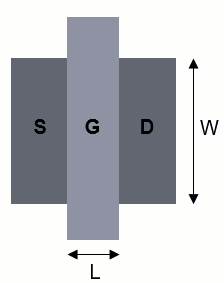
\includegraphics[width=.75\linewidth]{images/9.2}
			\caption{1 Finger MOS}
		\end{subfigure}
		\hfill
		\begin{subfigure}[t]{0.49\textwidth}
			\centering
			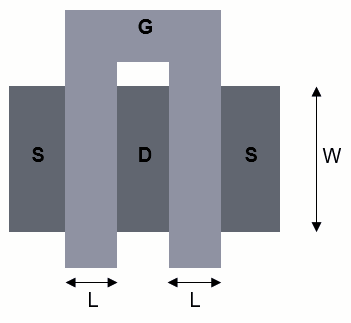
\includegraphics[width=1\linewidth]{images/10.3}
			\caption{2 Finger MOS}
		\end{subfigure}
		
		\caption{Multiple fingers layout (MOSFET transistor)}
		\label{fig:9}
	\end{figure}
	\subsubsection{Advantages}
	\begin{enumerate}
		\item 	\textbf{Improved RF performance:} Multi-finger design reduces gate resistance, leading to better high-frequency performance in RF circuits. 
		\item 	\textbf{Lower parasitic capacitance:} Dividing the gate into smaller sections can decrease parasitic capacitance, improving circuit speed and power efficiency. 
		\item \textbf{	Better matching:} When designing identical transistors with multiple fingers, the matching between them is often improved due to the similar layout and reduced variations.
	\end{enumerate}
	
	
	
	
	\newpage
	\section{Schematic Layout }
	\subsection{NOR Gate using 1 Finger MOS}
	\begin{figure}[H]
		\centering
		\includegraphics[width=0.65\linewidth]{"D:/DOWNLOAD 2024 V2/LATEX FILE/EEE_2214/EXP04_EEE2214/Images/1"}
		\caption{2 Input NOR-Gate using 1 Finger MOS}
		\label{fig:4}
	\end{figure}
	
	\subsection{OR Gate using 1 Finger MOS}
	
	\vspace{2cm}
	\begin{figure}[H]
		\centering
		\includegraphics[width=1\linewidth, height=0.7\textheight]{"D:/DOWNLOAD 2024 V2/LATEX FILE/EEE_2214/EXP04_EEE2214/Images/2"}
		\caption{2 Input OR-Gate using 1 Finger MOS and a CMOS}
		\label{fig:5}
	\end{figure}
	\subsection{NOR Gate using 2 Finger MOS}
	\vspace{1.5cm}
	\begin{figure}[H]
		\centering
		\includegraphics[width=0.7\linewidth]{"D:/DOWNLOAD 2024 V2/LATEX FILE/EEE_2214/EXP04_EEE2214/Images/3"}
		\caption{2 Input NOR-Gate using 2 Finger MOS }
		\label{fig:1}
	\end{figure}
	
	\newpage
	\subsection{OR Gate using 2 Finger MOS}
	\vspace{0.5cm}
	\begin{figure}[H]
		\centering
		\includegraphics[width=1\linewidth, height=0.6\textheight]{"D:/DOWNLOAD 2024 V2/LATEX FILE/EEE_2214/EXP04_EEE2214/Images/4"}
		\caption{2 Input OR-Gate using 2 Finger MOS and a CMOS }
		\label{fig:2}
	\end{figure}
	
	\section{Specification}
	\begin{table}[H]
		\centering
		\caption{MOSFET Dimensions for nMOS and pMOS Transistors}
		\label{tab:MOSFET_dimensions}
		\begin{tabular}{|c|c|c|c|c|}
			\hline
			\textbf{MOS} & \textbf{\begin{tabular}[c]{@{}c@{}}Width\\ ($\mu m$)\end{tabular}} & \textbf{\begin{tabular}[c]{@{}c@{}}Length\\ ($\mu m$)\end{tabular}} & \textbf{\begin{tabular}[c]{@{}c@{}}Width\\ ($\lambda$)\end{tabular}} & \textbf{\begin{tabular}[c]{@{}c@{}}Length\\ ($\lambda$)\end{tabular}} \\ \hline
			nMOS & 0.600 & 0.120 & 10 & 2 \\ \hline
			pMOS & 0.600 & 0.120 & 10 & 2 \\ \hline
		\end{tabular}
		
	\end{table}
	
	\begin{table}[H]
		\centering
		\caption{Parameters of Input Clock Signal for 1 Finger NOR-Gate and OR-Gate}
		% Sub-table (a)
		\begin{subtable}[t]{0.48\textwidth} % Adjusted width for each sub-table
			\centering
			\begin{tabular}{|c|c|c|}
				\hline
				\textbf{Parameter}          & \textbf{Value} & \textbf{Unit} \\ \hline
				High Level $(V)$            & 5.00           & $V$           \\ \hline
				Low Level $(V)$             & 0.00           & $V$           \\ \hline
				Time Low $(tl)$             & 0.225          & $ns$          \\ \hline
				Rise Time $(tr)$            & 0.001          & $ns$          \\ \hline
				Time High $(th)$            & 0.225          & $ns$          \\ \hline
				Fall Time $(tf)$            & 0.001          & $ns$          \\ \hline
			\end{tabular}
			\caption{Input clock signal of A} % Sub-table (a) caption
		\end{subtable}
		\hfil
		% Sub-table (b)
		\begin{subtable}[t]{0.48\textwidth} % Adjusted width for each sub-table
			\centering
			\begin{tabular}{|c|c|c|}
				\hline
				\textbf{Parameter}          & \textbf{Value} & \textbf{Unit} \\ \hline
				High Level $(V)$            & 5.00           & $V$           \\ \hline
				Low Level $(V)$             & 0.00           & $V$           \\ \hline
				Time Low $(tl)$             & 0.451         & $ns$          \\ \hline
				Rise Time $(tr)$            & 0.001          & $ns$          \\ \hline
				Time High $(th)$            & 0.451          & $ns$          \\ \hline
				Fall Time $(tf)$            & 0.001          & $ns$          \\ \hline
			\end{tabular}
			\caption{Input clock signal of B} % Sub-table (b) caption
		\end{subtable}
	\end{table}
	
	\begin{table}[H]
		\centering
		\caption{Parameters of Input Clock Signal for 2 Finger NOR-Gate and OR-Gate}
		% Sub-table (a)
		\begin{subtable}[t]{0.48\textwidth} % Adjusted width for each sub-table
			\centering
			\begin{tabular}{|c|c|c|}
				\hline
				\textbf{Parameter}          & \textbf{Value} & \textbf{Unit} \\ \hline
				High Level $(V)$            & 5.00           & $V$           \\ \hline
				Low Level $(V)$             & 0.00           & $V$           \\ \hline
				Time Low $(tl)$             & 0.225          & $ns$          \\ \hline
				Rise Time $(tr)$            & 0.001          & $ns$          \\ \hline
				Time High $(th)$            & 0.225          & $ns$          \\ \hline
				Fall Time $(tf)$            & 0.001          & $ns$          \\ \hline
			\end{tabular}
			
			\caption{Input clock signal of A} % Sub-table (a) caption
		\end{subtable}
		\hfil
		% Sub-table (b)
		\begin{subtable}[t]{0.48\textwidth} % Adjusted width for each sub-table
			\centering
			\begin{tabular}{|c|c|c|}
				\hline
				\textbf{Parameter}          & \textbf{Value} & \textbf{Unit} \\ \hline
				High Level $(V)$            & 5.00           & $V$           \\ \hline
				Low Level $(V)$             & 0.00           & $V$           \\ \hline
				Time Low $(tl)$             & 0.451         & $ns$          \\ \hline
				Rise Time $(tr)$            & 0.001          & $ns$          \\ \hline
				Time High $(th)$            & 0.451          & $ns$          \\ \hline
				Fall Time $(tf)$            & 0.001          & $ns$          \\ \hline
			\end{tabular}
			\caption{Input clock signal of B} % Sub-table (b) caption
		\end{subtable}
		
		
		
	\end{table}
	\begin{table}[H]
		\centering
		\caption{Parameters for Vdd+ and Vss- }
		\begin{tabular}{|c|c|c|}
			\hline
			\textbf{Parameter} & \textbf{Value} & \textbf{Unit} \\ \hline
			Vdd+               & 5.00           & $V $            \\ \hline
			Vss-               & 0.00           & $V$             \\ \hline
		\end{tabular}
		
	\end{table}
	
	\newpage
	\section{Output Waveshape }
	\subsection{NOR-Gate \& OR-Gate using 1 Finger MOS}
	\begin{figure}[H]
		\centering
		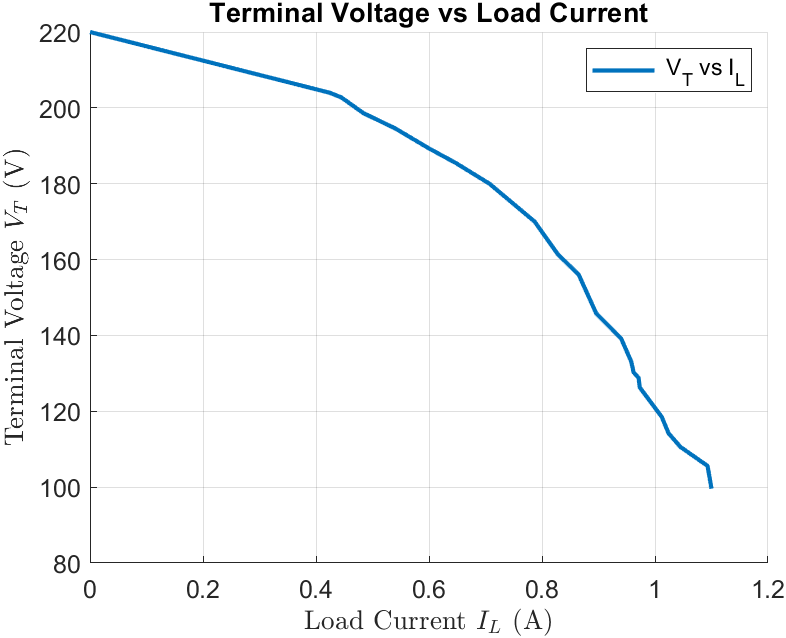
\includegraphics[width=1\linewidth, height=.40\textheight]{"D:/DOWNLOAD 2024 V2/LATEX FILE/EEE_2214/EXP04_EEE2214/Images/1.2"}
		\caption{Output Waveshape of 2 Input NOR-Gate using 1 Finger MOS}
		\label{fig:1nand}
	\end{figure}

	\begin{figure}[H]
		\centering
	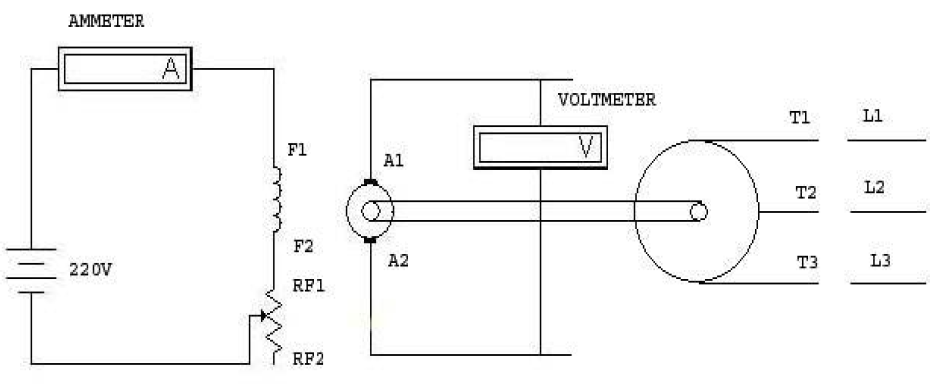
\includegraphics[width=1\linewidth, height=.40\textheight]{"D:/DOWNLOAD 2024 V2/LATEX FILE/EEE_2214/EXP04_EEE2214/Images/2.1"}
		\caption{Output Waveshape of 2 Input OR-Gate using 1 Finger MOS }
		\label{fig:1and}
	\end{figure}
	
	\newpage
	\subsection{NOR-Gate \& OR-Gate using 2 Finger MOS}
	
	\begin{figure}[H]
		\centering
		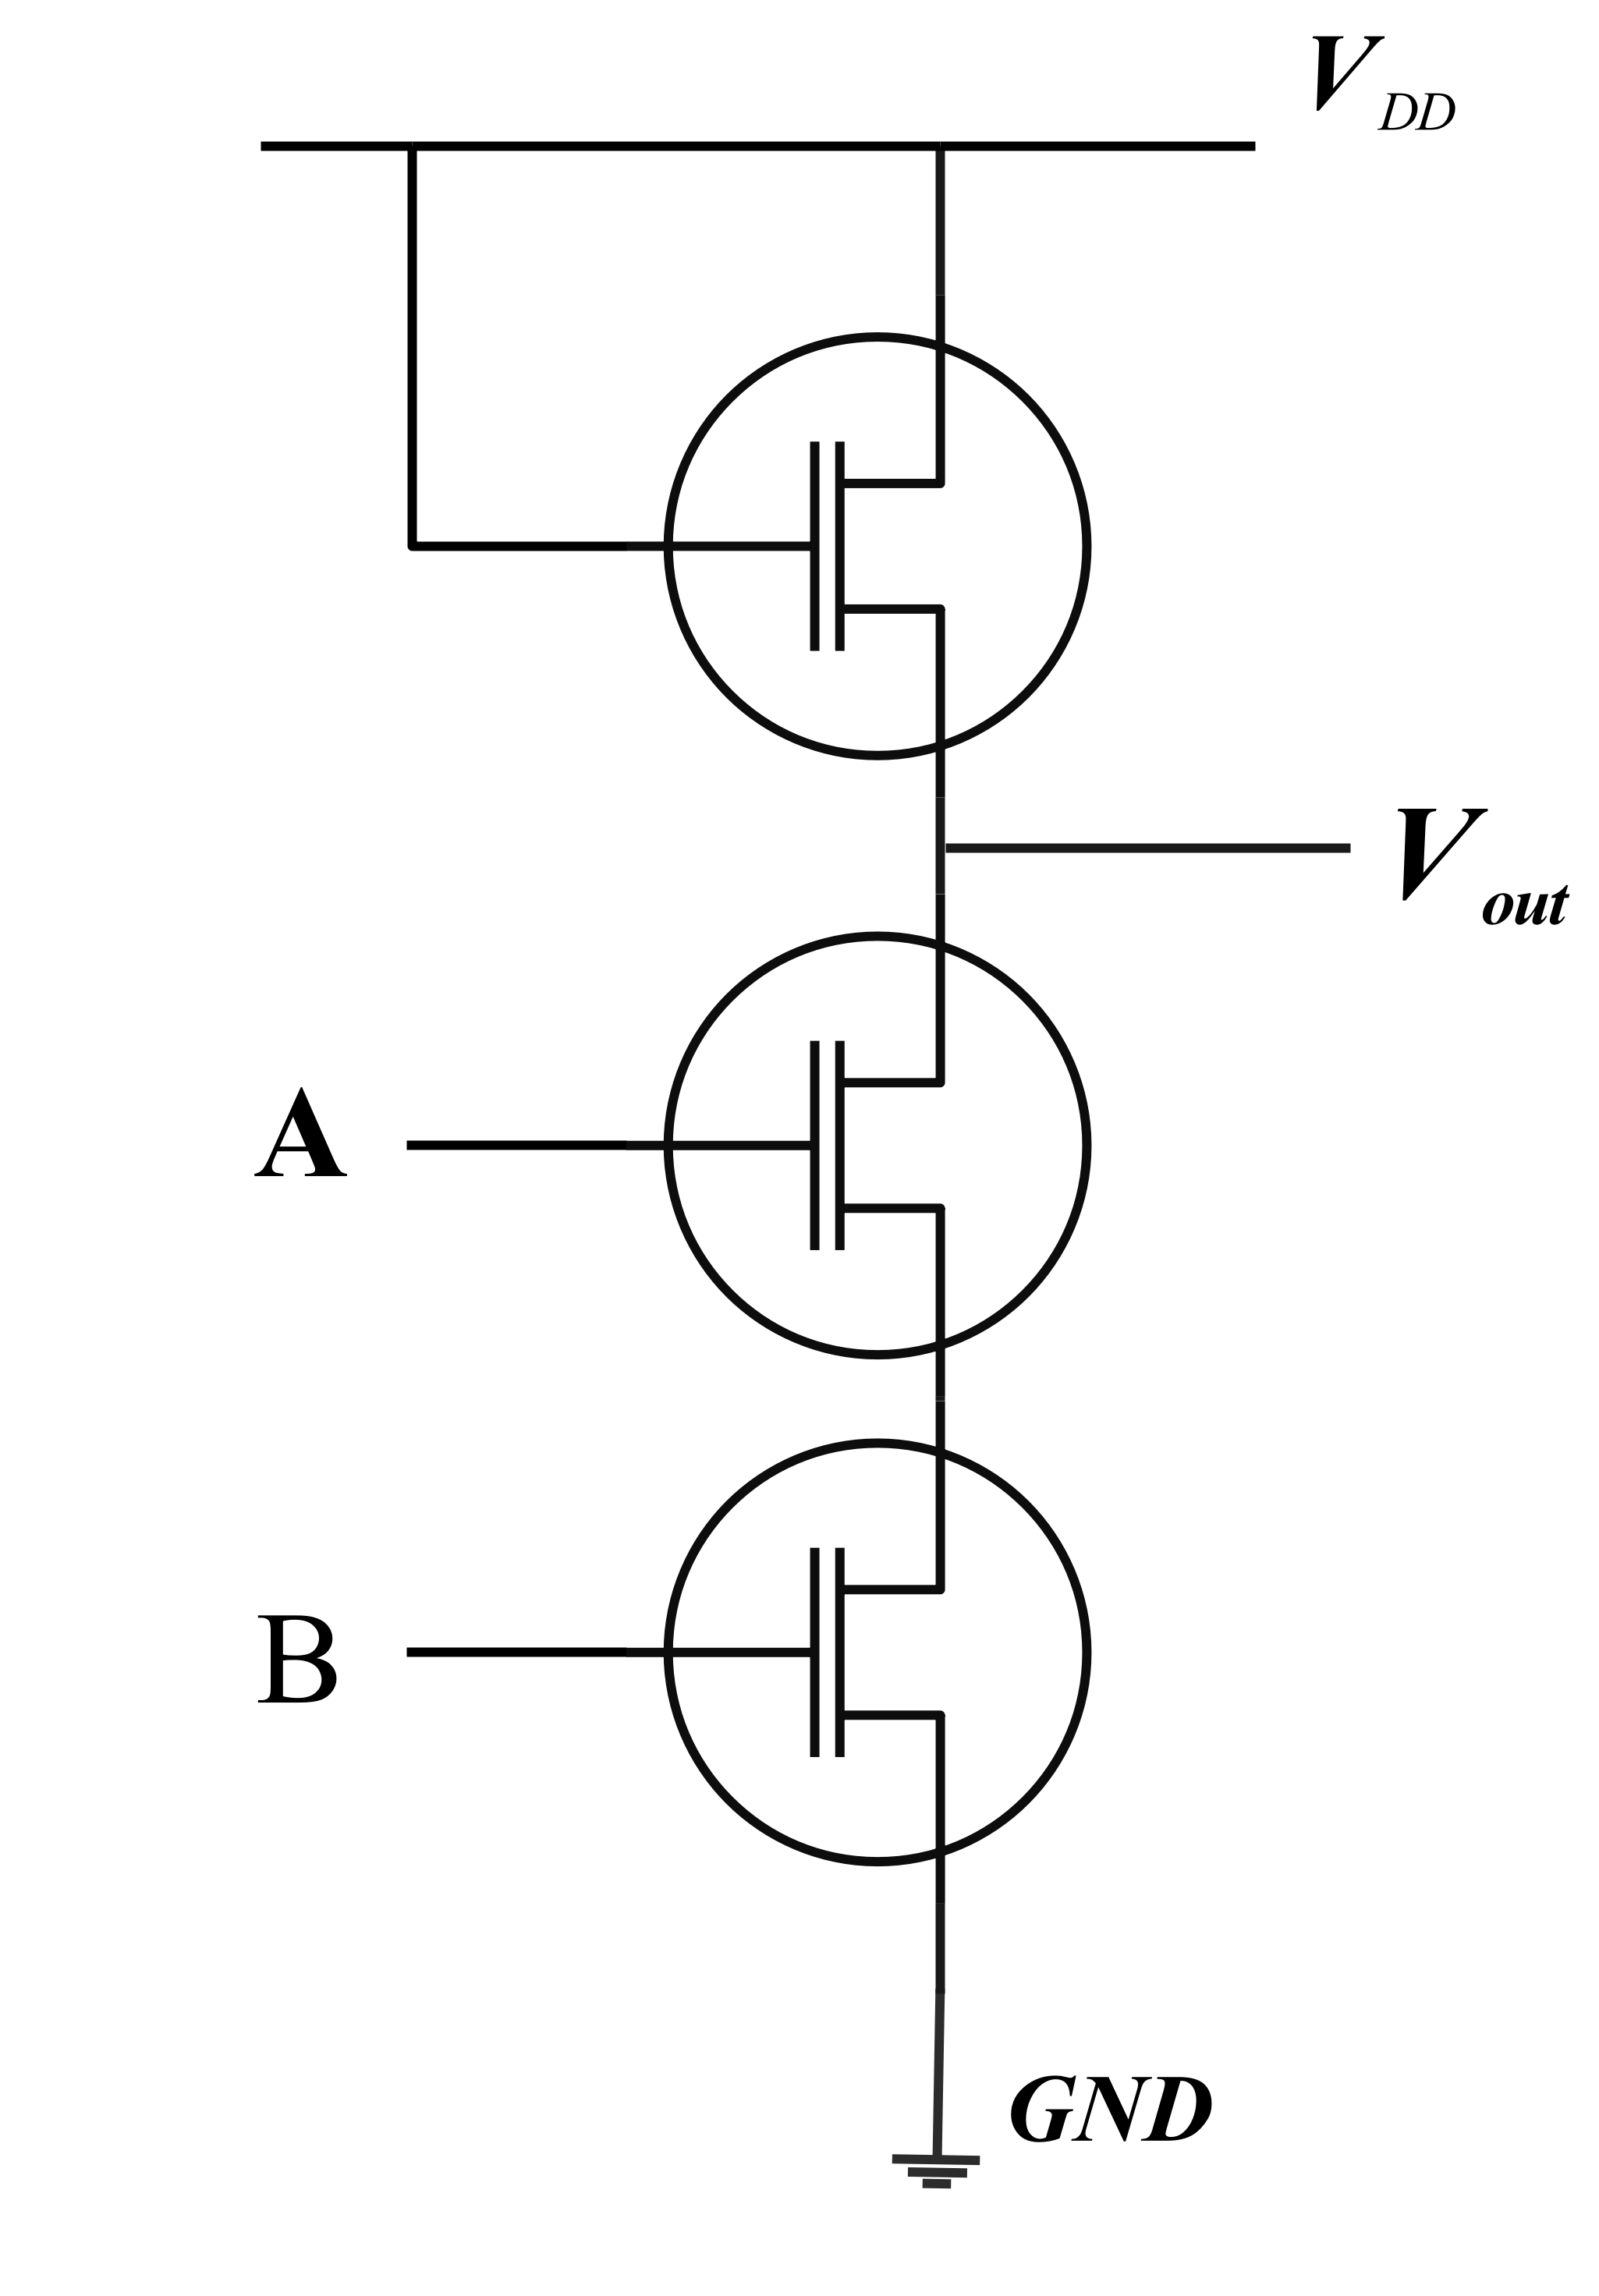
\includegraphics[width=1\linewidth, height=.40\textheight]{"D:/DOWNLOAD 2024 V2/LATEX FILE/EEE_2214/EXP04_EEE2214/Images/3.1"}
		\caption{Output Waveshape of 2 Input NOR-Gate using 2 Finger MOS}
		\label{fig:2nand}
	\end{figure}
	
	\begin{figure}[H]
		\centering
			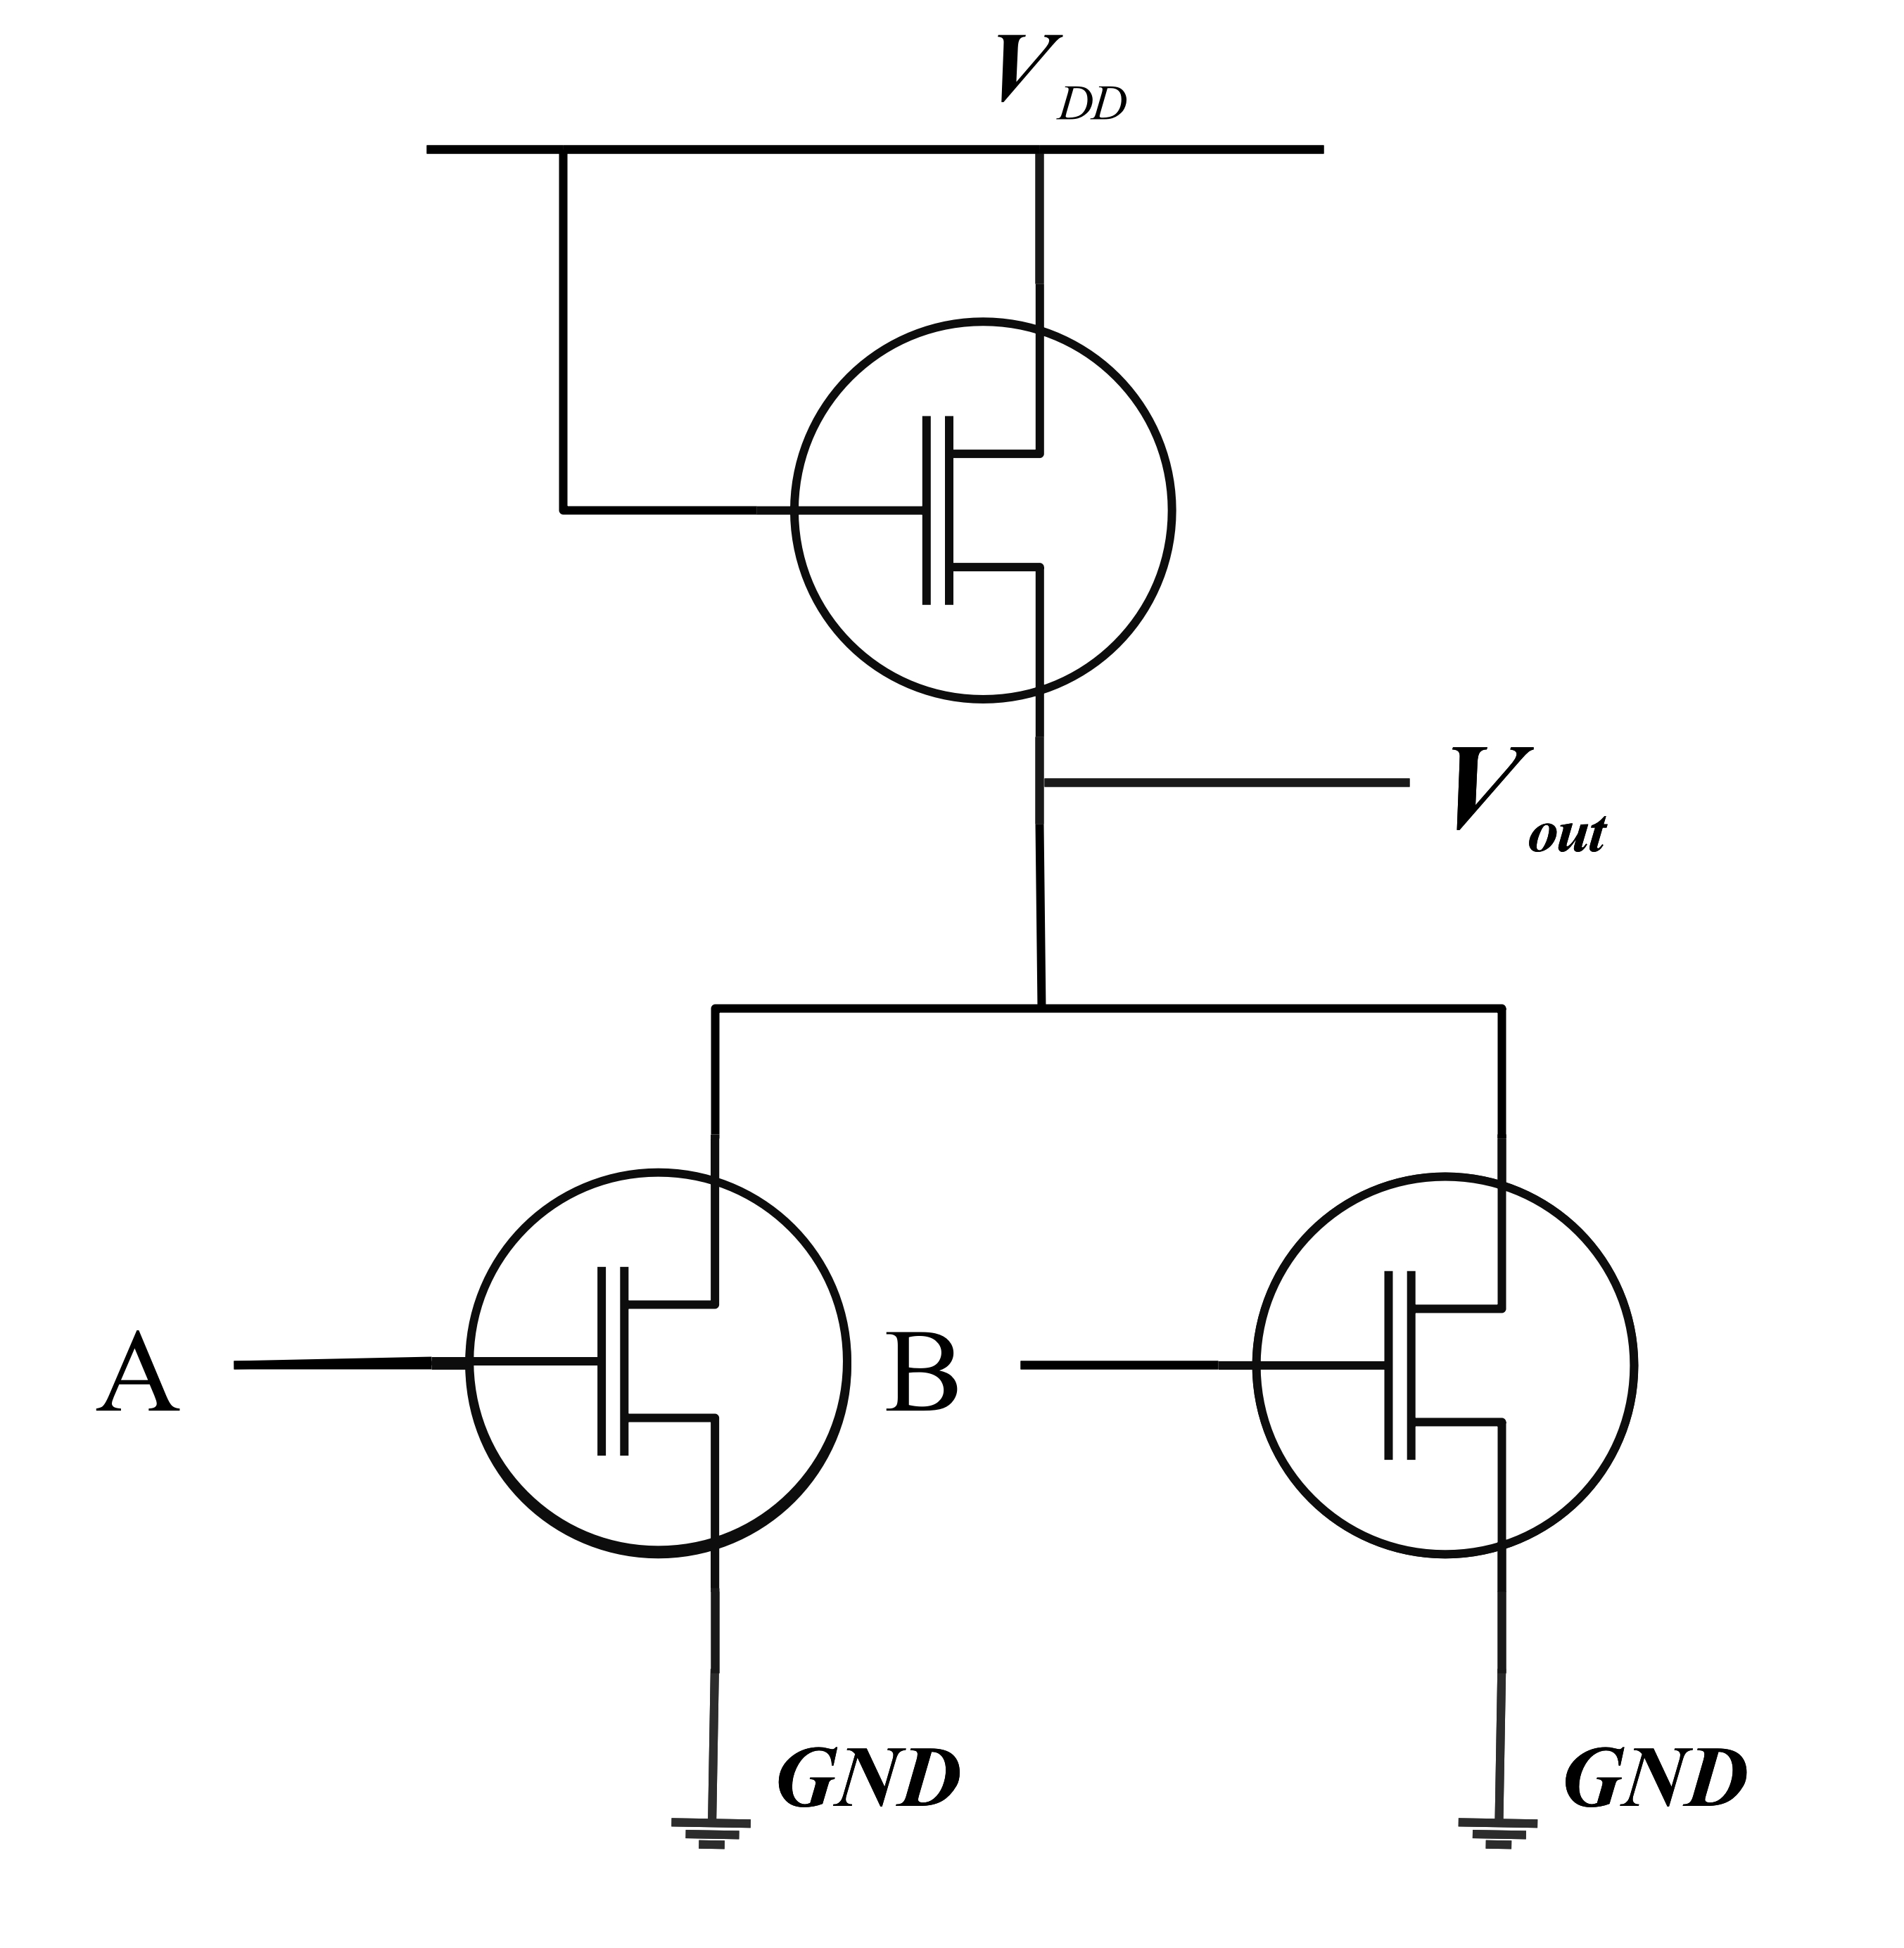
\includegraphics[width=1\linewidth, height=.40\textheight]{"D:/DOWNLOAD 2024 V2/LATEX FILE/EEE_2214/EXP04_EEE2214/Images/4.1"}
		\caption{Output Waveshape of 2 Input OR-Gate using 2 Finger MOS }
		\label{fig:2and}
	\end{figure}
	\newpage
	\section{Discussion}
	The characteristics of 2-input CMOS NOR and OR gates were analyzed based on the input signals \(A\) and \(B\) and the corresponding output signal \(F\). It was observed that the output of the OR gate was the complement of the output of the NOR gate for all input combinations, indicating that they are logical inverses of each other. The truth tables confirmed that when the OR gate output is logic high, the NOR gate output is logic low, and vice versa.\\
	
	During testing, the NOR gate exhibited some initial voltage fluctuations during state transitions, which were not present in the OR gate. This behavior in the NOR gate could be attributed to the charge and discharge dynamics of its pMOS and nMOS transistors during switching. Despite these fluctuations, both gates adhered to the expected logical behavior as outlined in the truth table.
	
	
	
\end{document}